\documentclass{report}
\usepackage[utf8]{inputenc}
\usepackage{textgreek}
\usepackage{gensymb}
\usepackage{graphicx}
\usepackage{listings}
\usepackage{amsmath}
\graphicspath{ {renders/} }



\begin{document}
\chapter{Simulation of X-Ray Pump Probe Experiments}

\section{Intensity Position Monitor}
At the X-Ray Pump Probe (XPP) beamline of SLAC National Accelerator Laboratory's LCLS, there are two beam monitors upstream of the sample position.
They are bespoke single shot intensity position monitors (IPM).
The first, IPM\textsubscript{2} is upstream of attenuator.
The second is IPM\textsubscript{3} is closer to the sample position, but suffers from less intense readings on the whole.
The IPM detectors both consist of four 10 mm square diodes (Figure \ref{ipm}).
Photons from the incident X-Ray beam are scattered by an amorphous silicon nitride (Si\textsubscript{3}N\textsubscript{4}) membrane.
Backscattered X-rays are collected on the detector panels and read out once per shot as the four intensity values $I_T, I_R, I_B, I_L$. 
The beam flux is then proportional to the sum of the panel readings, $I\propto \sum_{i\in T,R,B,L}I_i$. 
Furthermore, the position of them beam can be estimated from the panel readings as 

\begin{equation}\label{eq:position}
\begin{aligned}
Xpos &\propto \frac{I_R-I_L} {I_R + I_L} \\
Ypos &\propto \frac{I_T-I_B} {I_T + I_B}.
\end{aligned}
\end{equation}

\subsection{Estimating Si\textsubscript{3}N\textsubscript{4} Backscatter}
The X-ray beam incident on the silicon nitride film is polarized in the X plane. 
The differential scattering received at each point on the detector can be computed as the sum of elastic and inelastically scattered photons. 
The elastic scattering of photons from a free electron is referred to as Thompson scattering. 
For a polarized incident photon wavevector, the Thompson scattering is \cite{Hubbell1975-fl}

\begin{equation}
\bigg( \frac {d\sigma}{d\Omega} \bigg)_{Th} = r_0^2 \bigg(1 - \sin^2 \theta \cos^2 \phi \bigg),
\end{equation}



wherein $r_0$ is the classical radius of an electron. 
The angle $\theta$ is the angle between the incident beam wavevector and the scattered beam wavevector. 
It is very important to notice that this $\theta$ is not the same as the $\theta$ commonly encountered in the diffraction literature.
Following the notation of \cite{Hanson1986-ta}, this text refers to the diffraction angle as $\theta'=\pi - \theta$.
$\phi$ is the angle between the scattered beam wavevector and the incident beam polarization vector. 


In atoms, electrons are bound by nuclei and do not behave as free particles. 
In order to account for atomicity, the concept of the atomic form factor, $f$, was introduced. 
The form factor is a function of the scattering vector amplitude, $q = sin(\theta'/2)/\lambda$ and the atomic number of the atom, $Z$. 
$f$ can be used to compute the elastic scatter from the electrons in an atom which is referred to as Rayleigh scattering, 
\begin{equation}
\begin{aligned}
\label{formfactor}
\bigg( \frac {d\sigma}{d\Omega} \bigg)_R &= f^2(q, Z) \bigg( \frac {d\sigma}{d\Omega} \bigg)_{Th} \\
                                         &= f^2(q, Z)  r_0^2 \bigg(1 - \sin^2 \theta \cos^2 \phi \bigg).
\end{aligned}
\end{equation}
The atomic form factors are estimated from quantum mechnical calculations of the electron density for each atom and are tabulated in \cite{Hubbell1975-fl}. The tabulated form factors are reported for specific values of $q$ and are quadratically interpolated in practice.

In addition to elastic scattering, electrons will also exhibit inelastic scattering wherein there is some momemtum transfered from the photon to the electron. 
In inelastic scattering, the incident and scattered photons have different energies given by \cite{Heitler1954-vq}
\begin{equation}
k = \frac {k_0} {\mu + k_0(1 - \cos \theta)}. 
\end{equation}
Wherein $\mu = m_ec^2$ the rest mass energy of the electron and $k_0$ is the energy of the incident photon. 
For the case of polarized incident light, differential inelastic scattering of a free electron can be computed with the Klein-Nishina equation \cite{Klein1929-ic}
\begin{equation}
\label{compton}
\bigg( \frac {d\sigma}{d\Omega} \bigg)_{KN} = \frac {r_0^2} {4} \bigg(\frac{k}{k_0}\bigg)^2\bigg(\frac {k} {k_0} + \frac {k_0} {k} - 2 \sin^2 \theta \cos^2 \phi \bigg).
\end{equation}
The inelastic scattering of the free electron is known as Compton scattering. 
It can be adapted via an empirical function to yield the differential inelastic scattering for bound electrons in an atom.
This is called the atomic Compton scattering and it is attained by combining the Compton scattering for the free electron with the incoherent scattering function $S(q, Z)$.

\begin{equation}
\begin{aligned}
\bigg( \frac {d\sigma}{d\Omega} \bigg)_{aC} &= S(q, Z) \bigg( \frac {d\sigma}{d\Omega} \bigg)_{KN} \\
                                            &= S(q, Z)  \frac {r_0^2} {4} \bigg(\frac{k}{k_0}\bigg)^2\bigg(\frac {k} {k_0} + \frac {k_0} {k} - 2 \sin^2 \theta \cos^2 \phi \bigg).
\end{aligned}
\end{equation}

With these formulae in place, it is relatively straightfoward to compute the differential scattering for the IPM detector system. 
The detector target material is silicon nitride. 
To the scattering cross section of it is the weighted sum of the silicon and nitrogen atomic scattering dictated by the stoichiometry of the target, Si\textsubscript{3}N\textsubscript{4}.
\begin{equation} \label{eq:silicon_nitride}
\bigg( \frac {d\sigma}{d\Omega} \bigg)_{Si_3N_4} = \frac{3}{7}\bigg( \frac {d\sigma}{d\Omega} \bigg)_{Si} + \frac{4}{7}\bigg( \frac {d\sigma}{d\Omega} \bigg)_{N}.
\end{equation}

To compute the scattering onto the detector diodes, we simply need to convert the detector panel coordinates into spherical coordinates, $\theta$ and $\phi$ by the following equations

\begin{equation} \label{eq:spherical_transform}
\begin{aligned}
\theta &= \tan^{-1} {\bigg( \frac {\sqrt{(x-xpos)^2 + (y-ypos)^2}} {l} \bigg)} \\
\phi   &= \tan^{-1} \bigg(\frac {y - ypos} {x - xpos} \bigg).
\end{aligned}
\end{equation}
Pursuant to the spherical coordinate transformation \ref{eq:spherical_transform} and the differential formula for silicon nitride \ref{eq:silicon_nitride}, we can estimate the differential scattering cross section on the surface of the IPM panels \ref{ipm_heatmap}. 
It is then possible to numerically integrate over the detector surface subject to a simulated beam position. 
Position estimates from integrated panel intensities show excellent linearity with beam positions (figure \ref{fig:ipm_position}). 
At very large deflections, thousands of microns, the estimated beam positions become sublinear (figure \ref{fig:ipm_linearity}). 


\begin{figure}
\centering
\includegraphics[width=0.8\textwidth]{ipm.pdf}
\caption{Geometry of the Intensity Position Monitor. The IPM detector has four panels, here refered to as Top, Right, Bottom, and Left. The panels are 10 mm squares. The inner edge of the panels are found 10 mm from the centroid of the detector diode system. The X-ray beam position here is denoted by Xpos, Ypos in the cartesian detector coordinate system.}
\label{ipm}
\end{figure}

\begin{figure}
\centering
\includegraphics[width=0.8\textwidth]{theta.pdf}
\caption{Scattering off silicon nitride membrane to detector diode. 
Downstream of the detector by a distance z=l, is a silicon nitride film. 
At XPP, we believe that l is essentially 10 mm and that the film is 4 \textmu m thick. 
Photons scattered by the film are detected on the IPM panels. 
The scattering angle, $\theta$, is defined with respect to the forward scattering direction. 
Therefore, backscattered photons, as we detect here, are $\pi-\theta$  degrees from the Z axis. 
The backscattered photon shown above is the special case wherein $\phi=90$ degrees. 
However, in the general case, theta determines a circle in which the scattered photon can hit the detector system. 
The particular angle along that circle is given by $\phi$. 
}
\label{theta}
\end{figure}

\begin{figure}
\centering
\includegraphics[width=0.8\textwidth]{phi.pdf}
\caption{Relation between cartesian detector system and scattering angles $\theta$ and $\phi$}
\label{phi}
\end{figure}

\begin{figure} 
\centering
\includegraphics[width=0.8\textwidth]{ipm_heatmap.png}
\caption{Differential scattering of 1 \AA\ x-radiation onto the IPM panels. The beam position is marked by the circle at X=Y=0.}
\label{ipm_heatmap}
\end{figure}

\begin{figure} 
\centering
\includegraphics[width=0.8\textwidth]{ipm_position.png}
\caption{Beam position estimated from integrated IPM panel intensities according to \ref{eq:position}. Beam positions were generated by random draws from a gaussian centered at (0,0) (top left). Estimates of beam position }
\label{fig:ipm_position}
\end{figure}

\begin{figure} 
\centering
\includegraphics[width=0.8\textwidth]{ipm_edges.png}
\caption{The beam position estimates from the integrated IPM panels have a very large theoretical linear range. One hundred beam positions drawn from a gaussian centered at (0,0) with $\sigma_x=\sigma_y=2000\ \mu m$ and $\sigma_{xy}=0$.}
\label{fig:ipm_linearity}
\end{figure}

\section{Model for For Observed Reflection Intensities}
In order to generate, realistic "observations" of Bragg peak intensities, $I_h$, several factors must be considered. 
Chiefly, the reflection intensity is proportional to the square of the structure factor amplitude. 
However, the squared structure factor amplitude must be modified by several factors. 

\begin{equation}
I_h \propto F_h^2pfI_o
\end{equation}

The partiality, $p$, of a given observation is the fraction of that reflection which was observed on the detector. 
In X-FEL experiments, the X-ray pulses are too brief to move the detector during data collection. 
Therefore, all detector readouts only contain a portion of the 3-D reciprocal space volume of each reflection. 
For the moment, simulated partialities are simply drawn from a normal distribution. 
This approach finds some justification in the knowledge that Serial Femtosecond Crystallography essentially works by assuming partialities are sampled from a guassian. 
In addition to the partiality of the reflection, which is an intrinsic consequence of the crystal's mosaicity and alignment, the fraction of the incoming photons incident on the crystal needs to be taken into account. 
This is particularly important given that positional fluctions in the X-ray beam are often on the order of $\frac {1} {10}$ to $\frac {1} {5}$ of the linear dimension of the crystal. 
To compute the fraction of light incident on the crystal, $f$, we need to integrate over the X-ray beam intensity distribution. 
Here, we simply model the beam as a bivariate normal, $\mathcal{N}(\mu, \Sigma)$ with mean values, $\mu=\{xpos, ypos\}$ covariance matrix

\begin{equation}
\Sigma = 
\begin{bmatrix}
    \sigma_x^2 & 0 \\
    0 & \sigma_y^2 \\
\end{bmatrix}.
\end{equation}

Where the variances correspond to the linear aspect of the x-ray beam in the x and y dimensions. Generally, these numbers are in the 10s of microns. 
To compute f, we simply integrate $\mathcal{N}$ over the surface area of the crystal. 

\begin{equation}
\begin{aligned}
f = \int_A &\frac {1} {2\pi \sigma_x \sigma_y} e^{-\frac {1} {2} \big[ \frac {(x - xpos)^2}{\sigma_x^2} + \frac {(y - ypos)^2}{\sigma_y^2} \big]} \\
f = \frac {1} {4} \bigg[ &\bigg( Erf (\frac {xmin - xpos} {\sqrt {2} \sigma_x}) - Erf (\frac {xmax - xpos} {\sqrt {2} \sigma_x)} )\bigg)  \\
 &\bigg( Erf ( \frac {ymin - ypos} {\sqrt {2} \sigma_y}) - Erf (\frac {ymax - ypos} {\sqrt {2} \sigma_y}) \bigg)  \bigg]
\end{aligned}
\end{equation}

\section{Command Line Arguments for Data Simulator}
The data simulator in Gammastimator has been designed to be reasonably flexible with sane defaults. 
The only thing that necessarilly be provided by the end user are on and off structure factor amplitudes in CNS file format.
CNS was chosen, because it is the most sane plain text format that Phenix understands. 
The command signature for simulate.py is

\begin{lstlisting}
python simulate.py [options] Foff Fon out
\end{lstlisting}

A full list of options is given by the -h or -{}-help flag. 
Below, I will include a list of flags which I think might be routinely useful. 
The reader should appreciate that this is not an exhaustive list of the available parameters. 
\bigskip


\noindent
-{}-multiplicity [float : 20] 
\begin{quote}
    The multiplicity to which the dataset is sampled. 
    Internally simulate.py makes draws from the input data with replacement to build up the dataset of reflections. 
    Multiplicity says for the program to make multiplicity * the number of reflections in the input data.
\end{quote}

\noindent
-{}-missing [float : 0] 
\begin{quote}
    The fraction of missing reflections in the dataset. 
    A given reflection cannot always be integrated across all images at a given phi angle.
    This feature is meant to emulate the simple reality that reflections are often missing from some images.
    This will simply subsample the data before output. 
    Users may wish to do this themselves in post.
    Subsampling will speed up data generation.
    If you plan to subsample for testing anyway, you may want to use this option.
\end{quote}

\noindent
-{}-intensityscale [float : 2.0]
\begin{quote}
    The sum of the IPM readings for each simulated shot is drawn from a gamma distribution with probability density, 
    $p(x) = x^{k - 1} \frac {e^{-x/\theta}} {\theta^k \Gamma(k)}$. 
    The scale parameter, $\theta$, has been chosen to roughly approximate the empirical distribution of IPM readings from experiments at XPP. 
\end{quote}

\noindent
-{}-intensityshape [float : 0.2]
\begin{quote}
    The sum of the IPM readings for each simulated shot is drawn from a gamma distribution with probability density, 
    $p(x) = x^{k - 1} \frac {e^{-x/\theta}} {\theta^k \Gamma(k)}$. 
    The shape parameter, $k$, has been chosen to roughly approximate the empirical distribution of IPM readings from experiments at XPP. 
\end{quote}


\noindent
-{}-reflectionsperimage [int : 150]
\begin{quote}
    The mean number of reflections in an image. 
    Number of reflections are drawn from a gaussian with this mean truncated below minreflectionsperimage.
\end{quote}

\noindent
-{}-reflectionsperimagestd [int : 150]
\begin{quote}
    Number of reflections are drawn from a gaussian with this standard deviation truncated below minreflectionsperimage.
\end{quote}

\noindent
-{}-minreflectionsperimage [int : 50]
\begin{quote}
    The minimum number of reflections in an image. 
\end{quote}

\noindent
-{}-meanimages [int : 150]
\begin{quote}
    The mean number of phi angles per crystal. 
    Number of phi angles are drawn from a gaussian with this mean truncated below minimages.
\end{quote}

\noindent
-{}-minimages [int : 10]
\begin{quote}
    The minimum number of phi angles per crystal. 
    Number of phi angles are drawn from a gaussian with this mean truncated below minimages.
\end{quote}

\noindent
-{}-stdimages [int : 10]
\begin{quote}
    The standard deviation of the number of phi angles per crystal. 
    Number of phi angles are drawn from a gaussian with this mean truncated below minimages.
\end{quote}


\noindent
-{}-offreps [int : 4]
\begin{quote}
    The number of ``off" images with structure factor amplitutes sampled from Foff.
\end{quote}

\noindent
-{}-onreps [int : 4]
\begin{quote}
    The number of ``pumped" images with structure factor amplitutes sampled from Fon. 
\end{quote}

\noindent
-{}-sigintercept [float : 5]
\begin{quote}
    The error model in simulate.py is linear, such that $\sigma_I \approx aI + b$. 
    The sigintercept sets $b$ in the error model. 
\end{quote}

\noindent
-{}-sigslope [float : 0.03]
\begin{quote}
    The error model in simulate.py is linear, such that $\sigma_I \approx aI + b$. 
    The sigslope sets $a$ in the error model. 
\end{quote}

\noindent
-{}-partialitymean [float : 0.6]
\begin{quote}
    The average partiality of reflections.
    In simulate.py, partialities are drawn from a truncated gaussian centered at this value. 
    Partialities larger than 1. are rounded to 1. 
\end{quote}

\noindent
-{}-partialitystd [float : 0.2]
\begin{quote}
    The standard deviation of the partiality of reflections.
    In simulate.py, partialities are drawn from a truncated gaussian with this standard deviation.
    Partialities larger than 1. are rounded to 1. 
\end{quote}

\noindent
-{}-partialitymin [float : 0.2]
\begin{quote}
    The minimum partiality of reflections.
    In simulate.py, partialities are drawn from a truncated gaussian with values less than parialitymin rounded up to partialitymin.
    Partialities larger than 1. are rounded to 1. 
\end{quote}

\noindent
-{}-energy [float : 12398.0]
\begin{quote}
    The energy in electron volts of the X-ray beam used to image the crystal. 
    At the moment this is not used to calculate the observed intensities, but it is used in integrating scattering cross sections for the simulated IPM readings.
\end{quote}

\noindent
-{}-sigx [float : 10.0]
\begin{quote}
    In simulate.py, beam center X position is drawn from a gaussian with standard deviation sigx in \textmu m. 
\end{quote}

\noindent
-{}-sigy [float : 5.0]
\begin{quote}
    In simulate.py, beam center Y position is drawn from a gaussian with standard deviation sigx in \textmu m. 
\end{quote}


\noindent
-{}-divx [float : 50.0]
\begin{quote}
    In simulate.py, the X-ray beam is modeled as a gaussian with the standard deviation in the x axis determined by this flag.
\end{quote}

\noindent
-{}-divy [float : 100.0]
\begin{quote}
    In simulate.py, the X-ray beam is modeled as a gaussian with the standard deviation in the y axis determined by this flag.
\end{quote}

\noindent
-{}-sigheight [float : 10.0]
\begin{quote}
    In simulate.py, the vertical size of each crystal in \textmu m is drawn from a gaussian with this standard deviation.
\end{quote}

\noindent
-{}-height [float : 100.0]
\begin{quote}
    In simulate.py, the vertical size of each crystal in \textmu m is drawn from a gaussian with this mean. 
\end{quote}

\noindent
-{}-sigwidth [float : 10.0]
\begin{quote}
    In simulate.py, the horizontal size of each crystal in \textmu m is drawn from a gaussian with this standard deviation.
\end{quote}

\noindent
-{}-width [float : 100.0]
\begin{quote}
    In simulate.py, the horizontal size of each crystal in \textmu m is drawn from a gaussian with this mean. 
\end{quote}

\noindent
-{}-sigalign [float : 10.0]
\begin{quote}
    In simulate.py, the alignment of each crystal in \textmu m relative to the average beam center is drawn from a gaussian with this standard deviation and zero mean.
\end{quote}


\bibliographystyle{plain}
\bibliography{references}

\end{document}
